% This is samplepaper.tex, a sample chapter demonstrating the
% LLNCS macro package for Springer Computer Science proceedings;
% Version 2.20 of 2017/10/04
%
\documentclass[runningheads]{llncs}
%
\usepackage{graphicx}
% Used for displaying a sample figure. If possible, figure files should
% be included in EPS format.
%
% If you use the hyperref package, please uncomment the following line
% to display URLs in blue roman font according to Springer's eBook style:
% \renewcommand\UrlFont{\color{blue}\rmfamily}

\usepackage{multirow}
\usepackage{amsmath}
\usepackage{color}  %导言区调用color宏包
\usepackage{lipsum}
\usepackage{graphicx}% Include figure files
\usepackage{dcolumn}% Align table columns on decimal point
\usepackage{bm}% bold math
\usepackage{hyperref}%加入链接
\usepackage{geometry}
\geometry{margin=1in}
\hypersetup{
colorlinks=true,
linkcolor=red,
citecolor=green
}

\usepackage{marvosym} %通讯作者标


%\usepackage{fontspec} %字体设置包%
\usepackage{adjustbox} %表格居中

\begin{document}
%
\title{SLMamba: Synergizing Vision Mamba and Multi-scale Strip Large-kernel Convolutions for Medical Imaging}
\titlerunning{SLMamba: When Mamba Meets Strip and Large-kernel Convolution}

%
%\titlerunning{Abbreviated paper title}
% If the paper title is too long for the running head, you can set
% an abbreviated paper title here
%
\author{Zhibo Wang\and
Kaigui Wu\textsuperscript{\Letter} }
%
\authorrunning{Z. Wang et al.}
% First names are abbreviated in the running head.
% If there are more than two authors, 'et al.' is used.
%
\institute{
School of Computer Science, Chongqing University, Chongqing, 400044, China\\
\email{zhibowang@stu.cqu.edu.cn}\\
\email{kaiguiwu@cqu.edu.cn}}
%
\maketitle              % typeset the header of the contribution
%




\begin{abstract}
%The abstract should briefly summarize the contents of the paper in 15--250 words.

While Vision Mamba has emerged as a formidable alternative to Transformers for global context modeling, its efficacy in decoding complex medical structures remains limited. This paper introduces Strip Large-kernel Mamba (SLMamba), a novel hybrid architecture designed to bridge the gap between long-range dependency and directional feature refinement. Our core innovation lies in the Multi-scale Strip Large-kernel Convolutional Block (MSLCB), which replaces conventional decoders to explicitly capture the anisotropic features of slender organs. By integrating a Strip Large-kernel Gated Attention (SLGA) mechanism, the model effectively filters multi-scale noise while amplifying critical anatomical details. Extensive evaluations on Synapse and ACDC benchmarks demonstrate that SLMamba outperforms state-of-the-art models, particularly in small-object segmentation, achieving a DSC of 83.36\% and an impressive HD95 of 16.18 mm on Synapse.


\keywords{Medical Image Segmentation  \and Vision Mamba \and Strip Convolution \and Multi-scale Large-kernel Convolution.}
\end{abstract}



\section{Introduction}

Automated segmentation of anatomical structures in medical images, particularly computed tomography (CT), is a foundational task for computer-aided diagnosis, treatment planning and quantitative analysis\cite{ronneberger2015unet,milletari2016vnet,isensee2021nnu}. Convolutional Neural Networks (CNNs) long enjoys a dominant position due to their exceptional feature extraction capabilities. The U-Net architecture, based on CNNs, further establishes a new design paradigm and becomes the cornerstone for numerous models. Over time, however, the inherent limitation of CNNs in modeling long-range dependencies increasingly hinderes their application in medical practice. Researchers have addressed this issue by introducing the self-attention mechanism, and have built up high-performing models such as TransUNet\cite{chen2021transunet}, SwinUNet\cite{cao2021swinunet} and UNTER\cite{hatamizadeh2022unetr}. Nonetheless, the substantial computational overhead associated with self-attention imposes a significant burden on today's healthcare industry, creating a pressing demand for a new technological solution. This demand is satisfied by Vision Mamba, a novel architecture built upon selective state space models (SSMs)\cite{gu2023mamba,liu2024vmamba,zhu2024vim}.

Vision Mamba achieves competitive visual modeling capability with linear computational complexity, offering an efficient paradigm for capturing global context. Initial explorations have successfully integrated Mamba blocks as encoders in segmentation frameworks\cite{ruan2024vmunet,ma2024umamba}, demonstrating their potential. Nevertheless, a critical gap persists: The decoding layer depends on leveraging excellent contextual capabilities for generation, which is evidently not the inherent forte of Mamba. This explains why prevalent vision models built upon Mamba predominantly utilize it as the encoder, integrating it with a separate, non-Mamba decoder, as seen in architectures like Samba\cite{Smamba} and MaIL\cite{MaIL}.

To bridge this gap, we propose SLMamba, a novel hybrid architecture for efficient and accurate CT organ segmentation. Our core innovation lies in the first dedicated integration of a Vision Mamba-based encoder with a comprehensively enhanced convolutional decoder. Specifically, the encoder is constructed using hierarchical Vision Mamba (VSS) blocks to efficiently build global feature representations. For the decoder, a new Multi-scale Strip Large-kernel Convolutional Block (SLCB) and a Strip Large-Kernel Grouped Attention Gate (SLGAG) are applied to replace the standard components. Inspired by the success of large-kernel designs in modern CNNs \cite{liu2022convnext} and the efficiency of strip convolutions in capturing anisotropic structures \cite{hou2020strippooling}, the SLCB employs parallel strip convolutions and large-kernel depthwise separable convolutions to capture anisotropic features and broad contextual information simultaneously. The SLGAG refines the fusion of encoder and decoder features through skip connections using the same enhanced convolutional philosophy, ensuring that crucial spatial details and directional cues are preserved during upsampling.

The principal contributions of this work are threefold: 
\begin{enumerate}
\item We introduce SLMamba that synergistically combines the global modeling strength of a Vision Mamba encoder with the localized, detail-oriented capacity of a heavily augmented convolutional decoder. 
\item We design two novel core components SLCB and SLGAG that systematically incorporate strip and large-kernel convolutions to better address the geometric and textural characteristics of medical organs. 
\item Extensive experiments on Synapse and ACDC demonstrate that our SLMamba achieves state-of-the-art performance with markedly improved efficiency, offering a compelling solution for practical medical image analysis.
\end{enumerate}


\section{Related Works}

This section contains a brief review of related works in the realm of medical image segmentation before introducing Mamba and then give a short review of SSMs.

\subsection{Medical image segmentation}

The evolution of medical image segmentation has been fundamentally driven by one core challenge: the trade-off between efficient local feature extraction and effective global context modeling. Early vision architectures predominantly relied on Convolutional Neural Networks (CNNs)\cite{ronneberger2015unet}, with the U-Net framework establishing the de facto standard. However, while Convolutional Neural Networks (CNNs) exhibit high computational efficiency and benefit from strong inductive biases—such as translation invariance and locality \cite{lecun2015deep, he2016resnet}—the intrinsic locality of standard convolution operations inherently restricts their capacity to model long-range spatial dependencies \cite{wang2018nonlocal}. Research has demonstrated that the effective receptive field of CNNs actually grows much slower than theoretically expected, often failing to encompass sufficient global context in deep layers \cite{luo2016erf}. Consequently, this structural constraint limits the performance of CNN-based models when processing complex scenes or anatomical structures with significant scale variations, where capturing global relational information is critical for resolving local ambiguities \cite{dosovitskiy2020vit, chen2021transunet}.

To address the limitations of long-range dependency modeling, researchers introduced Vision Transformers (ViTs) \cite{dosovitskiy2020vit}, which catalyzed a paradigm shift in computer vision. By replacing standard convolutions with the self-attention mechanism, Transformers demonstrate a remarkable capacity to model global contextual information, thereby enabling the network to perceive the entire image field comprehensively. The advent of the Transformer architecture has spurred the development of various high-performance medical image segmentation models. For instance, TransFuse \cite{zhang2021transfuse} employs a parallel-branch encoder to process local and global features simultaneously, effectively fusing CNN-based spatial details with Transformer-based global context. Swin-UNet \cite{cao2023swin} further enhances computational efficiency and adaptability for dense prediction tasks by utilizing hierarchical feature maps and shifted window attention. Additionally, DS-TransUNet \cite{lin2022ds} incorporates a dual-stream architecture to capture multi-scale representations from patches of varying sizes through parallel Swin Transformer blocks. Other notable contributions, such as SegFormer \cite{xie2021segformer} and Medical Transformer (MedT) \cite{valanarasu2021medical}, have further demonstrated the robustness of attention-driven frameworks in handling complex anatomical variations.

However, this enhancement in representation learning entails a significant drawback: the computational complexity of the self-attention mechanism scales quadratically with the input sequence length. This imposes a substantial memory and computational burden, particularly when processing high-resolution 2D or volumetric 3D medical images \cite{vaswani2017attention, hatamizadeh2022unetr}. To mitigate these constraints, researchers have increasingly turned toward hybrid architectures that balance efficiency with performance \cite{xie2021cotr}. A seminal example is TransUNet \cite{chen2021transunet}, which integrates a CNN-based encoder for robust local feature extraction and subsequently utilizes a Transformer at the bottleneck to model long-range global dependencies. By synergizing local spatial hierarchies with global contextual perception, TransUNet achieves superior performance compared to many pure Transformer-based counterparts. This paradigm underscores the profound potential of hybrid designs, which has become a prevalent strategy in contemporary medical vision frameworks. Consistent with this trend, our SLMamba is also built upon a hybrid architecture, aiming to optimize the trade-off between local precision and global context.

\subsection{State Space Model}

State Space Models (SSMs), deeply rooted in classical control theory and signal processing, provide a robust mathematical framework for modeling dynamical systems \cite{kalman1960new}. These models characterize the evolution of a system's latent states through linear ordinary differential equations (ODEs) or their discrete-time counterparts, offering a principled methodology for processing both continuous and discrete sequences \cite{gu2021efficiently}. Historically, SSMs have been recognized for their rigorous theoretical foundations and their innate capacity to capture long-range dependencies with linear computational complexity—a property that stands in stark contrast to the quadratic scaling inherent in the self-attention mechanism of Transformers \cite{gu2023mamba, vaswani2017attention}. By effectively mapping input sequences to hidden representations through a recursive or convolutional formulation, SSMs have emerged as a highly efficient alternative for modeling extensive temporal or spatial contexts \cite{gu2020hippo, fu2022hungry}.

The application of State Space Models (SSMs) to deep learning accelerated significantly with the introduction of the Structured State Space Sequence model (S4) \cite{gu2021efficiently}. S4 integrated the HiPPO (Hidden Information Processing for Preserving Online Trajectories) initialization framework for long-range memory with a structured, linear time-invariant (LTI) formulation, facilitating highly efficient parallel training and demonstrating remarkable performance on extensive sequence modeling tasks \cite{gu2020hippo}. However, a critical limitation of standard S4 and similar LTI-SSMs is their intrinsic time-invariant property—their state-transition parameters remain fixed and strictly independent of the input data \cite{fu2022hungry}. This structural rigidity fundamentally restricts their capacity to perform context-dependent reasoning or to selectively focus on salient information within a complex sequence, an imperative requirement for tasks involving dense and heterogeneous visual representations \cite{gu2023mamba}.

To overcome these inherent constraints, the groundbreaking selective state space model, notably Mamba \cite{gu2023mamba}, was introduced. The core innovation of Mamba lies in parameterizing the SSM transition matrices as functions of the input, thereby incorporating a data-dependent selection mechanism. This allows the model to dynamically propagate or attenuate information based on the current context, significantly enhancing its representation capacity for information-dense data such as natural language and medical imagery \cite{zhu2024vim, liu2024vmamba}. By maintaining the computational efficiency of linear scaling while introducing this selective capability, Mamba-based architectures have emerged as a high-performance alternative to Transformers, effectively bridging the gap between global receptive fields and computational economy in complex vision tasks \cite{ruan2024vmunet, ma2024umamba}.





\begin{figure*}
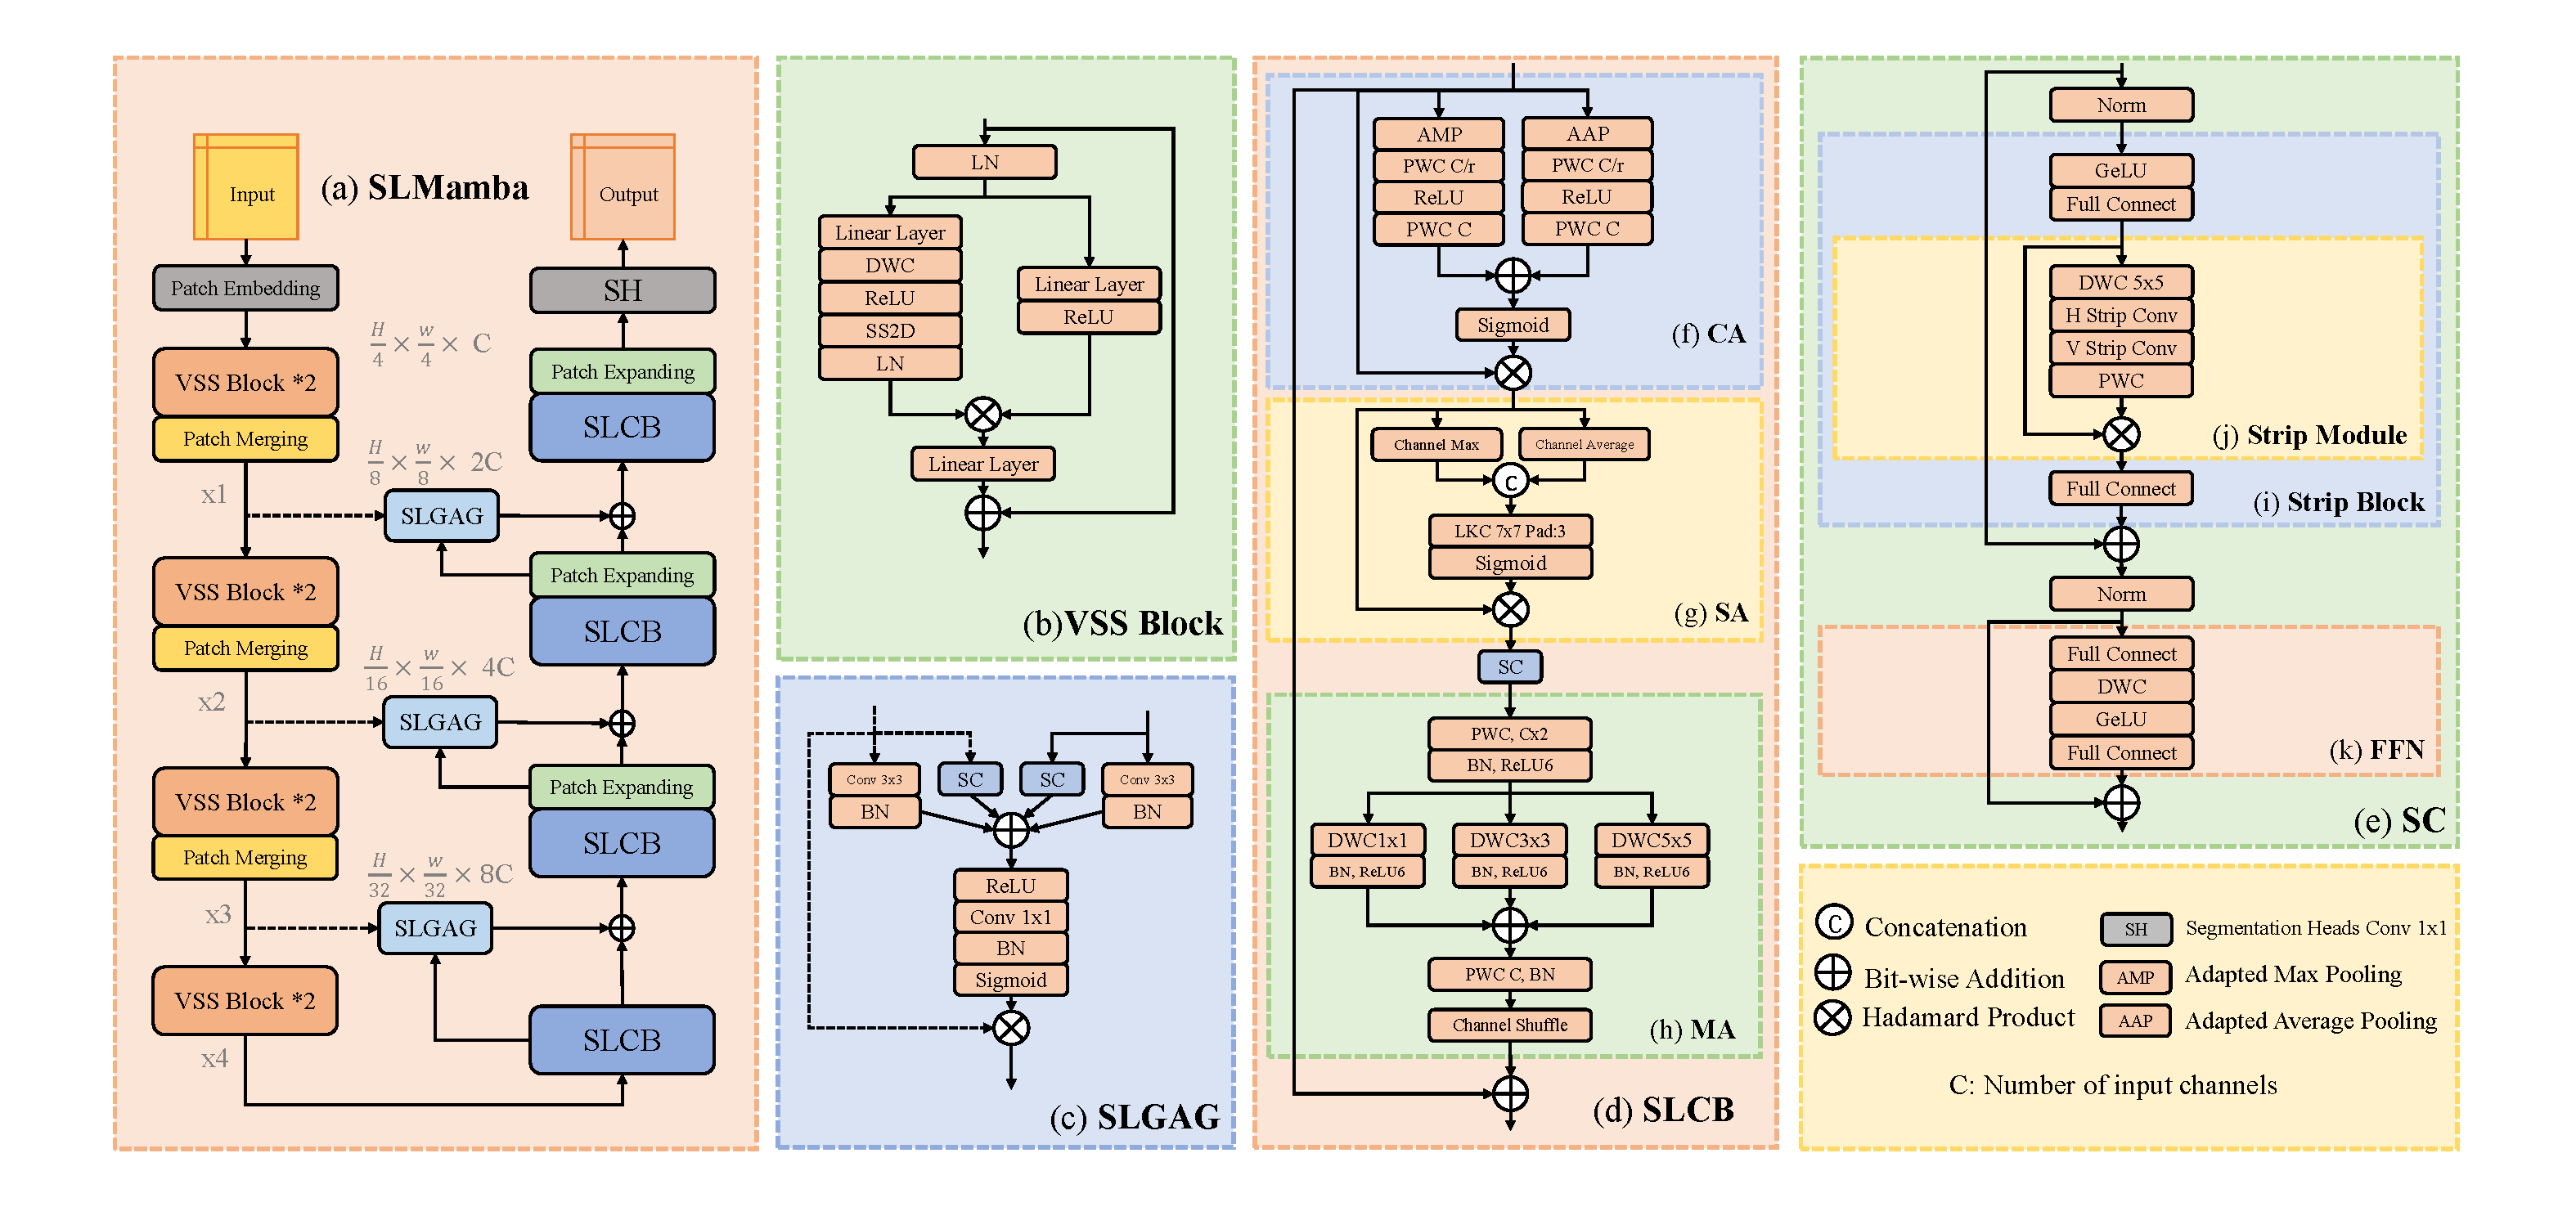
\includegraphics[width=\linewidth]{Figures/SLMamba.pdf}
\caption{
	(a) The overall architecture of SLMamba. 
	(b) VSS Block is the main construction of our encoder. 
	(c) Strip Large-kernel grouped attention gate(SLGAG) can enhance features from skip connections.
	(d) Multi-scale Strip Large-kernel convolutional block(SLCB), progressing patches in all dimensions to further enhance features, is the main component of our decoder.
	(e) Strip convolutional block(SC). 
	(f) Channel attention block(CA). 
	(g) Spatial attention block(SA).  
	(h) Multi-scale attention block(MA). 
	(i) Strip block.
	(j)	Strip module.
	(k) Feed-Forward Network(FFN). 
} \label{figure1}
\end{figure*}





\section{Methodology}

This section will first introduce the overall architecture of SLMamba, followed by a detailed description of each individual module used within it, including various technical principles, implementation details, and parameter settings.

\subsection{SLMamba}

As depicted in Figure \textcolor{red}{\ref{figure1}} (a), the overall architecture of SLMamba is presented, which is based on U-Shape-Network\cite{ronneberger2015unet}. Specifically, SLMamba comprises a Patch Embedding layer as initial processing, four-stage VSS Blocks\cite{liu2024vmamba,gu2023mamba} as the encoder, four-stage SLCBs as the decoder, a SH layer as final projection and SLGAGs as skip connections.

Firstly, in the Patch Embedding layer input image is divided from 
$x=R^{H\times W\times 3} $
into
${x}{'}\in {R}^{\frac{H}{4} \times \frac{W}{4} \times C}$, each patch is non-overlapping and the size is $4 \times 4$, subsequently mapping the dimensions of the image to C. Before entering the encoder layers, ${x}{'}$ will be normalized.

For the encoder, eight VSS Blocks are employed distributed across four stages, with each stage comprising two VSS Blocks. A patch merging operation is applied at the end of the first three stages to downsample the spatial dimensions of the input features while simultaneously doubling the channel capacity \cite{liu2021swin}. Consequently, the channel counts for the four stages are denoted as [C, 2C, 4C, 8C].

Similarly, the decoder utilizes four Multi-scale Strip Large-kernel Convolutional Blocks (SLCBs) to progressively refine the hierarchical pyramid features extracted from the encoder via skip connections (i.e., x1, x2, x3, and x4, as illustrated in Figure 1) \cite{lin2017feature}. Furthermore, a patch expanding operation is employed following the initial three SLCBs to progressively restore the spatial resolution \cite{cao2023swin}. The channel counts for the decoder stages follow the reverse order: [8C, 4C, 2C, C].

To bridge the semantic gap between the encoder and decoder, three Strip Large-Kernel Grouped Attention Gates (SLGAGs) are integrated within the skip connections \cite{oktay2018attention}. The features that are upsampled in the patch expanding layer are subsequently element-wise added to the refined outputs from the corresponding SLGAGs.

Finally, a Segmentation Head (SH) layer is applied to project the fused features and produce the final segmentation output.

\subsection{VSS Block}

As depicted in Figure \textcolor{red}{\ref{figure1}} (b), the VSS Block, derived from VMamba\cite{zhu2024vim,liu2024vmamba}, is the core module of our encoder. Firstly, the input patches $x$ are layer normalized, then split into two branches, where one branch performs global modeling but loses local features, and the other branch preserves local features.

The front branch firstly processes the input patches through a linear layer $LL(.)$ and a depthwise separable convolution $DWC(.)$, with an activation function $R(.)$ at the end. We then feed the patches into $SS2D(.)$ for future feature extraction. Finally, the features are layer normalized by $LN(.)$ and await output patches from the other branch.

As the front branch loses local features through global modeling, the local features will be preserved in the other branch, where patches will only undergo a linear layer $LL(.)$ and an activation function $R(.)$.

The outputs from both branches then undergo a bit-wise multiplication(Hadamard Product) after passing through another linear layer $LL(.)$. Finally, the merged features are added bit-wise to the initial input $x$.

The $VSS(.)$ can be formulated as in Equation \textcolor{red}{1}:
\begin{scriptsize} 
\begin{align} 
  VSS(x) = x + SS2D\left(\text{LN}\left(\text{DWC}\left(\text{LL}(x)\right)\right)\right) \otimes \sigma\left(\text{LL}(x)\right)
\end{align} 
\end{scriptsize}



\subsection{Strip Large-kernel grouped attention gate (SLGAG)}

We introduce a new strip large-kernel group attention gate (SLGAG) to enhance the activation of relevant features while suppressing irrelevant ones. 

As shown in Figure \textcolor{red}{\ref{figure1}} (c), SLGAG accepts two inputs, $g$ and $x$, from a patch expanding layer in the decoder and a patch merging layer that is one level higher than the patch expanding layer; both inputs have the same size to ensure bit-wise addition operates correctly. SLGAG processes $g$ and $x$ using a $3 \times 3$ convolution ($Cnv_{3\times 3}(\cdot)$) and a strip convolution ($SC(\cdot)$) to extract features. These convolved features are then batch-normalized using $BN(\cdot)$ and merged via bit-wise addition. The merged feature map is activated by a ReLU layer $R(\cdot)$. Afterward, a $1 \times 1$ convolution ($Cnv_{1\times 1}(\cdot)$) is applied to obtain a single-channel feature map. Then the single-channel feature map will pass through a $BN(\cdot)$ and an activation function $\sigma(\cdot)$ to successfully yield the attention coefficients. 

Finally, initial input $x$ and the activated single-channel feature map enter a bit-wise multiplication to produce the attention-gated feature.

The $SLGAG(.)$ can be formulated as in Equation \textcolor{red}{2}: 
\begin{scriptsize}
\begin{align}\nonumber
	SLGAG(g,x) = x \otimes \sigma(BN(Cnv_{1\times 1}(R(SC(g) + BN(Cnv_{3\times 3}(g)) + \\SC(x) + BN(Cnv_{3\times 3}(x))))))
\end{align}
\end{scriptsize}

\subsection{Multi-scale Strip Large-kernel convolutional block (SLCB)}

We introduce a new multi-scale strip large-kernel convolutional block as depicted in Figure \textcolor{red}{\ref{figure1}} (d). Our SLCB contains a channel attention block (CA) that finds out most relevant channel, a spatial attention block (SA) that find out the most relevant feature maps, a strip convolution block (SC) that enhances feature extraction capacity for tiny details, and a multi-scale attention block (MA) that enhances contextual relationships among all of the features.

\textbf{Channel Attention Block (CA)}\cite{woo2018cbam}: As depicted in Figure \textcolor{red}{\ref{figure1}} (f), the input patches $x$ first enter the channel attention (CA) module and are then split into two branches, where $x$ undergo adaptive max pooling\cite{he2014spatial} ($AMP(\cdot)$) and adaptive average pooling ($AAP(\cdot)$)\cite{he2014spatial} respectively, to extract the most significant feature per channel from the entire feature map. For each pooled feature map, two point-wise convolution blocks\cite{lin2013network} are applied: $PWC_{C/r}(\cdot)$ (with $r=16$) to reduce the number of channels and $PWC_C(\cdot)$ to recover it, with an activation function $R(\cdot)$ in between. The two pooled feature maps are then combined via bit-wise addition before passing through an activation function $\sigma(\cdot)$. Finally, a bit-wise multiplication is applied between the combined feature map and the initial input $x$ to get the final output.

The $CA(.)$ can be formulated as in Equation \textcolor{red}{3}:
\begin{scriptsize}   
\begin{align}
  CA(x) = x \otimes \sigma(PWC_{C}(R(PWC_{C/r}((AMP(x))))) + \nonumber
  \\PWC_{C}(R(PWC_{C/r}(AAP(x)))))
\end{align}
\end{scriptsize}

\textbf{Spatial Attention Block (SA)}\cite{woo2018cbam}: As depicted in Figure \textcolor{red}{\ref{figure1}} (g), following a design similar to that of the CA module, the input patches $x$ first undergo max pooling ($CH_{max}(\cdot)$) and average pooling ($CH_{average}(\cdot)$) in two separate branches along the channel dimension to capture local features. The outputs are then concatenated before being fed into a large-kernel convolution layer $LKC(\cdot)$ (i.e., kernel size is $7\times7$ and padding is 3), where local contextual relationships among the features are enhanced. Finally, the concatenated feature maps are passed through an activation function $\sigma(\cdot)$ and bit-wise multiplied (Hadamard product) with the initial input $x$.

The $SA(.)$ can be formulated as in Equation \textcolor{red}{4}:
\begin{scriptsize}   
\begin{align}
  SA(x) = x \otimes \sigma(LCK([CH_{max}(x); CH_{average}(x)]))
\end{align}
\end{scriptsize}

\textbf{Multi-scale Attention Block (MA)}: As depicted in Figure \textcolor{red}{\ref{figure1}} (h), the input patches $x$ first undergo channel expansion via a point-wise convolution $PWC_{C\times 2}(\cdot)$ (with an expansion factor of 2), followed by batch normalization $BN(\cdot)$ and an activation function $R6(\cdot)$ (ReLU6\cite{howard2017mobilenets}). Then, the patches are separately passed through three depthwise separable convolution layers ($DWC(\cdot)$) with different kernel sizes to capture multi-scale and multi-resolution contexts (the number and size of the kernels are configurable). After the features from different channels are summed, a channel shuffle layer\cite{zhang2018shufflenet} $CSF(\cdot)$ will be applied to enhance cross-channel relationships. The shuffled feature maps are then passed through another point-wise convolution $PWC_C(\cdot)$ to recover the original number of channels, followed by batch normalization $BN(\cdot)$. Finally, the normalized feature maps are added bit-wise to the initial input $x$.

The $MA(.)$ can be formulated as in Equation \textcolor{red}{5}:
\begin{scriptsize}   
\begin{align}
  MA(x)=x+BN(PWC_{C}(CSF(\sum_{}^{}DWC_{k_i}(R6(BN(PWC_{C\times2}(x)))))))
\end{align}
\end{scriptsize}



% Synapse 可视化 %
\begin{figure*}[h]
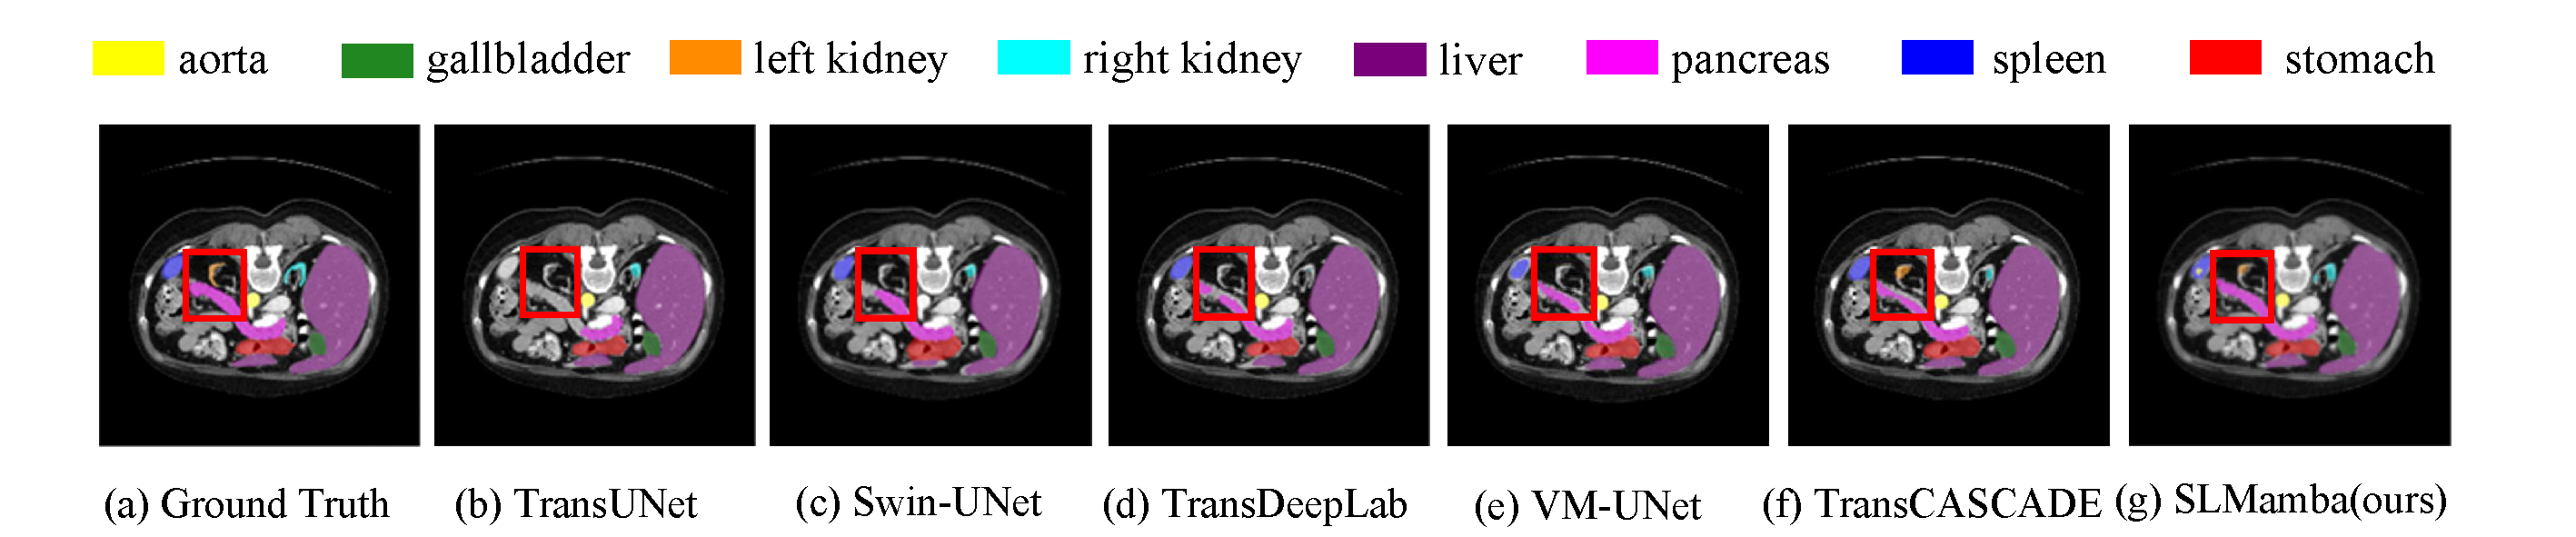
\includegraphics[width=\linewidth]{Figures/Synapse.pdf}
\caption{
	Qualitative results on Synapse datasets are shown .The red rectangular box highlights incorrectly segmented polyps by SOTA methods.
} \label{figure2}
\end{figure*}

% Synapse 结果 %
\begin{table*}[h]
\footnotesize
\centering
\label{f1}
\begin{tabular}{l|cc|cccccccc}\hline
Methods & DICE$\uparrow$ & HD95$\downarrow$ &Aor.& Gal. &Kid.(L) &Kid.(R) &Liv. &Pan. &Spl. &Sto. \\\hline

UNet\cite{ronneberger2015unet} & 70.11& 44.69& 84.00 &56.70& 72.41& 62.64& 86.98& 48.73& 81.48& 67.96 \\
AttnUNet\cite{oktay2018attention}& 71.70& 34.47& 82.61& 61.94& 76.07& 70.42& 87.54& 46.70& 80.67& 67.66 \\
TransUNet\cite{chen2021transunet} & 77.48 &31.69& 87.23 &63.13 &81.87 &77.02 &94.08 &55.86& 85.08& 75.62	\\
SSFormer\cite{wang2022stepwise}& 78.01& 25.72&  82.78& 63.74& 80.72& 78.11& 93.53& 61.53& 87.07& 76.61 \\
PolypPVT\cite{dong2021polyp} & 78.08& 25.61&  82.34& 66.14& 81.21& 73.78& 94.37& 59.34& 88.05& 79.4 \\
Swin-UNet\cite{cao2021swinunet} & 79.56 & 21.55 & 85.47 &66.53 &83.28 &79.61& 94.29 &56.58& 90.66& 76.60	\\
MT-UNet\cite{wang2022mixed} & 78.59 &26.59& 87.92& 64.99& 81.47& 77.29& 93.06& 59.46& 87.75& 76.81\\
MEW-UNet\cite{ruan2022mew} & 78.92& 16.44& 86.68& 65.32& 82.87& 80.02& 93.63& 58.36& 90.19& 74.26\\
PVT-CASCADE\cite{rahman2023medical} & 81.06& 20.23& 83.01& 70.59& 82.23& 80.37& 94.08& 64.43& 90.1& 83.69 \\
TransDeepLab\cite{azad2022transdeeplab} & 80.16& 21.25& 86.04& 69.16& 84.08& 79.88& 93.53& 61.19& 89.00& 78.40\\
VM-UNet\cite{ruan2024vmunet} & 81.08& 19.21& 86.40& 69.41& 86.16& 82.76& 94.17& 58.80& 89.51& 81.40 \\
TransCASCADE\cite{rahman2023transcascade} & 82.68 &17.34 & 86.63 &68.48& 87.66& 84.56& \textbf{94.43}& \textbf{65.33}& 90.79& 83.52\\
\hline
SLMamba(ours) & \textbf{83.36}& \textbf{16.18}& \textbf{88.43}& \textbf{70.94}& \textbf{88.57}& \textbf{84.79}& 94.33& 64.59& \textbf{91.23}& \textbf{84.01} \\\hline
\end{tabular}
\caption{Results on Synapse Multi-Organ Segmentation. DICE scores are reported for individual organs. $\uparrow$ denotes higher the better, $\downarrow$ denotes lower the better. The best results are in bold.}
\label{table1}
\end{table*}




\subsection{Strip Convolution Block (SC)}

Strip Convolution Block (SC)\cite{hou2020strip,liu2023slak,chu2021active} is integrated into our SLMamba to address the limitations of traditional square-kernel convolutions in capturing elongated and curvilinear anatomical structures.

SC is designed as shown in Figure \textcolor{red}{\ref{figure1}} (e). The input $x$ first passes through a layer normalization, a fully connected layer, and a GELU activation function\cite{hendrycks2016gelu}. The normalized patches $x'$ then enter the Strip Module, which is the core part of SC depicted in Figure \textcolor{red}{\ref{figure1}} (j).

In the Strip Module, a depthwise convolution with a large kernel (i.e., $5 \times 5$) is first applied to extract local contextual features. Then, two sequential depthwise convolutions with strip-shaped kernels (i.e., kernel size is $1 \times N$ and $N \times 1$) are used to better capture objects of high aspect ratios, followed by a pointwise convolution.

The output of the Strip Module, denoted as $Z$, undergoes an bit-wise multiplication (Hadamard product) with $x'$, yielding $Z'$, which then passes through an bit-wise addition with $x$ after a fully connected layer. Subsequently, the fully connected output is added bit-wise to $x$ again, producing $Y$. Next, the normalized $Y$ is passed through a feed-forward network where features are refined and enhanced, followed by another bit-wise addition with the normalized $Y$, yielding the final output $SC(X)$.


\subsection{Loss Function}

To optimize the SLMamba for high-precision medical image segmentation, we employ a hybrid loss function, denoted as $L_{total}$, which synergistically combines Soft Dice Loss and Focal Loss.

The rationale behind this design is two-fold. First, Soft Dice Loss is utilized to maximize the spatial overlap between the segmented masks and the ground truth, effectively mitigating the issues caused by the severe class imbalance inherent in medical datasets (e.g., small lesion areas versus large background regions). Second, to address the challenge of hard-to-classify pixels near anatomical boundaries, Focal Loss is integrated. By introducing a modulating factor $(1 - p_t)^\gamma$, Focal Loss reshapes the standard cross-entropy loss to down-weight easy examples and focus the model's learning capacity on ambiguous regions and sparse foreground pixels.

The objective function is formulated as in Equation \textcolor{red}{6}:

\begin{footnotesize}   
\begin{align}
  L_{total} = \lambda_{dice} L_{Dice} + \lambda_{focal} L_{Focal}
\end{align}
\end{footnotesize}

where $\lambda_{dice}$ and $\lambda_{focal}$ are hyper-parameters representing the weighting coefficients for each component. In our experiments, we empirically set $\lambda_{dice} = 1$ and $\lambda_{focal} = 1$ to maintain a balanced gradient flow throughout the backpropagation process, ensuring both global structural consistency and local boundary sharpness.

\section{Experiments}

This section will present the details of implementation followed by a comparative analysis of our SLMamba against SOTA methods, including the performance of the complete model on the datasets and the details of the ablation study.

\subsection{Implementation details}

To evaluate the proposed SLMamba, comprehensive experiments are conducted on two widely adopted public benchmarks: the Synapse multi-organ segmentation dataset \cite{landman2015miccai} and the Automated Cardiac Diagnosis Challenge (ACDC) dataset \cite{bernard2018deep}. During preprocessing, all images are uniformly resized to a spatial resolution of $224 \times 224$. To mitigate the risk of overfitting and enhance the generalization capability of the model, standard data augmentation techniques, including random flipping and random rotation, are employed. We set the batch size to 32 and employ AdamW optimizer \cite{loshchilov2017decoupled} with the initial learning rate configured to $1 \times 10^{-5}$ and weight decay configured to $1 \times 10^{-3}$. Furthermore, a cosine annealing learning rate scheduler \cite{loshchilov2016sgdr} is applied to dynamically adjust the learning rate, utilizing a maximum of 50 iterations and a minimum learning rate of $1 \times 10^{-5}$. The entire training process spans 300 epochs. For quantitative assessment, two primary evaluation metrics are utilized: the Dice Similarity Coefficient (DSC) to measure region-based overlap \cite{milletari2016v}, and the 95\% Hausdorff Distance (HD95) to evaluate boundary-based accuracy \cite{huttenlocher1993comparing}. All experiments are implemented using the PyTorch framework and executed on a single NVIDIA RTX 5090 GPU.










\subsection{Experimental Results}

SLMamba have compared with many state-of-the-art models with different type of architecture on Synapse and ACDC datasets. Pure CNN models like UNet\cite{ronneberger2015unet}. Pure Transformer models like Swin-UNet\cite{cao2021swinunet,cao2023swin}. Pure Mamba models like VM-UNet\cite{ruan2024vmunet}. Hybrid architecture models like TransUNet\cite{chen2021transunet} that uses CNN and Transformer. And other SOTA models such as TransCASCADE\cite{rahman2023transcascade} and so on. The later result details indicate our SLMamba achieves best among the SOTAs.



\subsubsection{Results on Synapse Multi-Organ Segmentation}

Results of experiments on Synapse are presented in Table \textcolor{red}{\ref{table1}}. Among SOTAs our SLMamba achieves the best performance, boasting a mean DICE score of 83.56 and a mean HD95 of 16.18, surpassing TransCASCADE\cite{rahman2023transcascade} and VM-UNet\cite{ruan2024vmunet}. There are two facts help our model, one is Mamba encoder costs less resources but predicts more precisely, the other one is our SLMamba employs large-kernel and strip convolution that successfully enhance capacity of feature extraction. Figure \textcolor{red}{\ref{figure2}} shows visual results of some SOTA models on Synapse segmentation. Evidently, several SOTA models exhibit misclassifications. TransUNet\cite{chen2021transunet}, Swin-UNet\cite{cao2021swinunet}, TransDeepLab\cite{azad2022transdeeplab} and VM-UNet\cite{ruan2024vmunet} miss left kidney. TransUNet\cite{chen2021transunet} and Swin-UNet\cite{cao2021swinunet} even lost very big part of pancreas. A similar limitation is observed in TransDeepLab\cite{azad2022transdeeplab} but not serious like the former two. Our SLMamba performs best, especially in segmentation on tiny and slender organs such as both right and left kidney.




\subsubsection{Results of ACDC Segmentation}

Results of experiments on ACDC are presented in Table \textcolor{red}{\ref{table2}}. Our model achieves the best performance with a mean DICE score of 92.81. Figure \textcolor{red}{\ref{figure2}} presents visual results of SOTA models performing on ACDC segmentation. SLMamba get a better performance than Swin-UNet\cite{cao2021swinunet}, TransUNet\cite{chen2021transunet} and TransDeepLab. Swin-UNet\cite{cao2021swinunet} predict incorrectly, missing the middle part of left ventricle. TransUNet\cite{chen2021transunet} similarly but miss the left part. TransDeepLab\cite{azad2022transdeeplab} miss parts of Myo and captures wrong extra parts for left ventricle. Additionally, VM-UNet\cite{ruan2024vmunet}  and TransCASCADE\cite{rahman2023transcascade} predict around correctly, however, not smoothly or precisely as our SLMamba.


% ACDC可视化 %
\begin{figure*}[h]
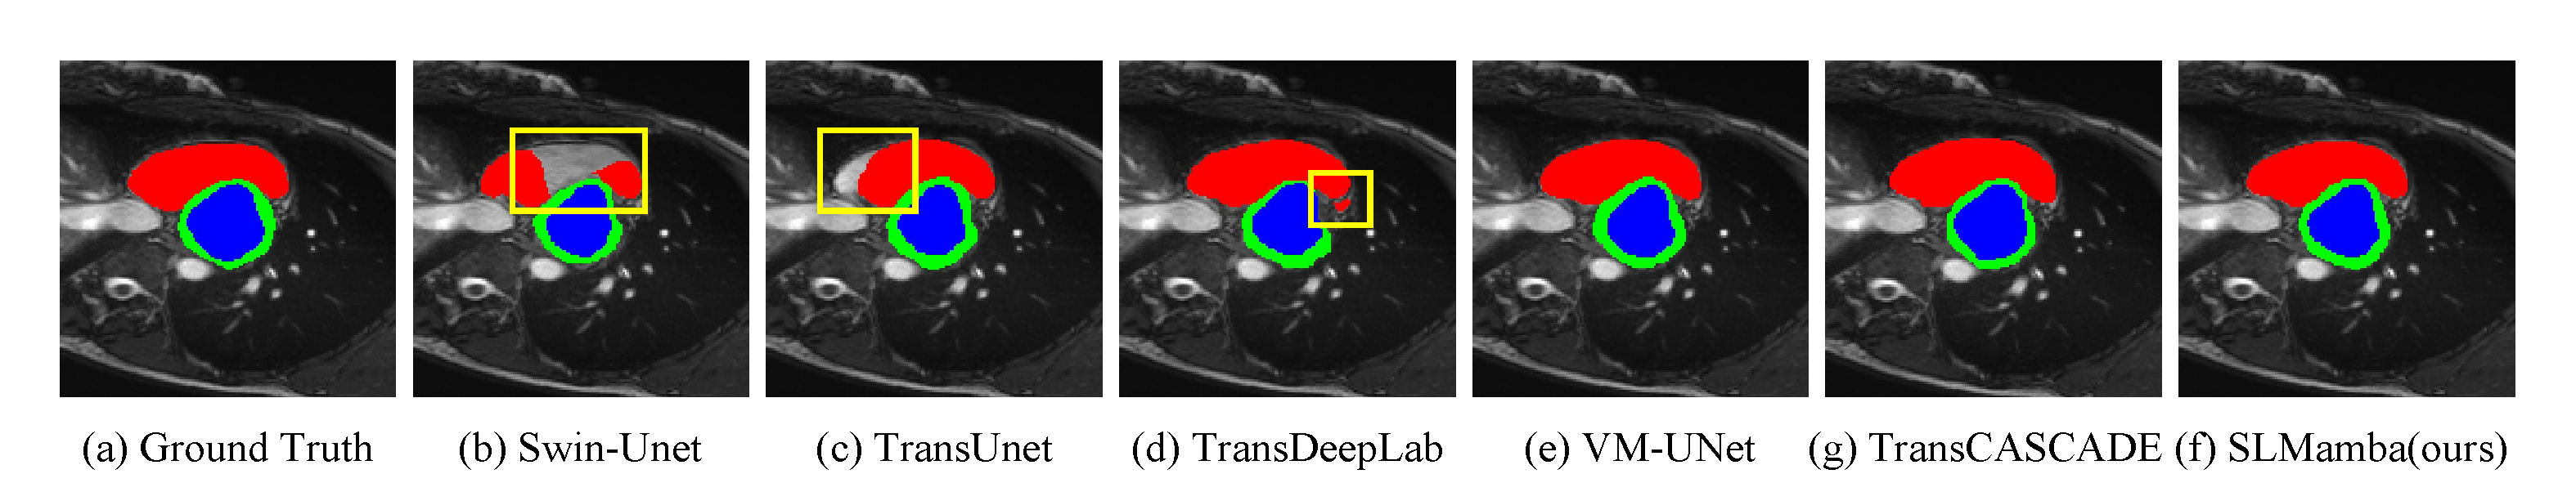
\includegraphics[width=\linewidth]{Figures/ACDC.pdf}
\caption{
	Qualitative results on ACDC datasets are shown .Red represents the right ventricle, blue represents the left ventricle,and green represents the myocardium. The yellow rectangular box highlights incorrectly segmented polyps by SOTA methods.
} \label{figure3}
\end{figure*}


% ACDC 结果 %
\begin{table}[h]
\footnotesize
\centering
\begin{tabular}{l|c|ccc}\hline
Methods & DICE$\uparrow$  &RV &Myo& LV\\\hline
TransUNet\cite{chen2021transunet} & 89.71& 86.67& 87.27& 95.18 \\
SwinUNet\cite{cao2021swinunet} & 90.00& 88.55& 85.62& 95.83 \\
HiFormer\cite{heidari2023hiformer} & 90.12& 91.06& 84.54& 94.77 \\
TransDeepLab\cite{azad2022transdeeplab} & 90.41& 91.45& 84.54& 95.23 \\
MT-UNet\cite{wang2022mixed} & 90.43& 86.64& 89.04& 95.62 \\
MISSFormer\cite{huang2022missformer} & 90.86& 89.55& 88.04& 94.99 \\
ParaTransCNN\cite{sun2024paratranscnn} & 91.31& 92.76& 85.84& 95.34 \\
VM-UNet\cite{ruan2024vmunet} & 91.63& 90.25& 89.14& 95.50 \\
TransCASCADE\cite{rahman2023transcascade} & 92.12& 90.65& 89.68& 96.02 \\
\hline
SLMamba(ours) & \textbf{92.81} & \textbf{91.52} & \textbf{90.58} &\textbf{96.53} \\\hline
\end{tabular}
\caption{ Results on ACDC. DICE scores($\%$)are reported for individual organs.$\uparrow$ denotes higher the better. The best results are in bold.}
\label{table2}
\end{table}



% 编码器消融实验 %
\begin{table}[h]
\small
\centering
\begin{tabular}{l|cc|c}\hline
\multirow{2}{*}{Methods} & \multicolumn{2}{c|}{Synapse} & ACDC \\\cline{2-4}
& DICE$\uparrow$ & HD95$\downarrow$ & DICE$\uparrow$ \\\hline
SLCNN & 81.93 &18.27& 89.94\\
SLTrans & 82.76 & 16.62 & 91.05\\\hline
SLMamba & \textbf{83.36} & \textbf{16.18} & \textbf{92.81} \\\hline
\end{tabular}
\caption{Results of how different encoders affect performance of segmentaion on Synapse and ACDC datasets. $\uparrow$ denotes higher the better, $\downarrow$ denotes lower the better. The best results are in bold.}
\label{table3}
\end{table}

\subsection{Ablation Studies}

%\subsubsection{Structure Ablation}

\subsubsection{Effect of Mamba Encoder}

To understand the effect of different encoders, a set of experiments are conducted on the Synapse and ACDC datasets. Two extra version of SLMamba, SLCNN and SLTrans by replacing the encoder using CNN and Transformer, have been built up tp be compared. Table \textcolor{red}{\ref{table3}} shows the experimental results. Our SLMamba with vision mamba encoder have achieved the best scores on both the Synapse and ACDC datasets, surpassing SLCNN and SLTrans. Such results are completely in line with our expectations. The capability of CNNs in processing image features can no longer meet the surging demands, and their performance falls short when compared to Transformers and Mamba. However, Transformers also have limitations, as an excessive amount of data not only leads to a sharp increase in parameter counts but may also negatively impact segmentation results. In contrast, the Mamba encoder's ability to compress data in long-sequence\cite{yu2024mambaout} tasks is likely the key factor that enables it to outperform Transformers.


% SLGAG 消融实验 %
\begin{table}[h]
\footnotesize
\centering
\begin{tabular}{l|ccc|c}\hline
\multirow{2}{*}{Methods} & \multicolumn{3}{c|}{Synapse} & ACDC \\\cline{2-5}
& DICE$\uparrow$ & HD95$\downarrow$ &Kid.(L) & DICE$\uparrow$ \\\hline
No-SLGAG & 81.80 & 18.47 &83.97  & 90.79\\\hline
SLMamba & \textbf{83.36} & \textbf{16.18} &\textbf{88.57}  & \textbf{92.81} \\\hline
\end{tabular}
\caption{Results of Ablation Experiment of how Strip Large-kernel Group Attention Gate(SLGAG) affects on Synapse and ACDC datasets. $\uparrow$ denotes higher the better, $\downarrow$ denotes lower the better.}
\label{table4}
\end{table}

% MA 卷积核策略 消融实验%
\begin{table*}[h]
\small
\centering
\begin{tabular}{l|cccccccccc}\hline
\multirow{2}{*}{Methods} & \multicolumn{10}{c}{Kernel Strategies} \\\cline{2-11}
& [1] & [3] & [5] & [1,3] & [3,5] & [3,3,3] &[1,3,5]& [5,5,5] &[3,5,7] &[1,3,5,7]  \\\hline
Synapse& 83.11& 82.93& 82.64& 83.02& 83.25& 82.73 & \textbf{83.36}& 82.98& 83.15& 83.20 \\
ACDC & 91.14 &91.94 & 91.89 &92.28& 91.93& 92.35& \textbf{92.81}& 92.32& 92.12& 92.43\\
\hline
\end{tabular}
\caption{Results of different depthwise convolution kernel strategies effect on Synapse and ACDC. In $[k_{1},k_{2},...,k_{n}]$, $k_{i}$ means size of each kernel, $\sum_{1}^{n}k_{i}$ means total number of the kernels. The best results are in bold.}
\label{table5}
\end{table*}


\subsubsection{Effect of SLGAG}

To observe the actual effectiveness of our SLGAG, one specifical experiment has been designed by removing the skip connections composed of SLGAG from SLMamba and use unprocessed skip connections instead, comparing this variant with our existing SLMamba on the Synapse and ACDC datasets. The experimental results are shown in Table \textcolor{red}{\ref{table4}}. The SLMamba with SLGAG achieves higher scores than the model without SLGAG, particularly demonstrating a significant lead in segmentation tasks involving small and elongated structures, such as the left kidney on the Synapse dataset. This indicates that the strip convolutions in our SLGAG can effectively capture relatively small and elongated features.


\subsubsection{Effect of Convolution Kernel Size in MA}

A series of experiments have been designed to evaluate the performance of the SLCB module. Specifically, experiments on the Synapse and ACDC datasets are conducted, with variable number and size of depthwise convolution kernels within the MA module. There are several strategies, including the use of a single $3 \times 3$ kernel, multiple $3 \times 3$ kernels, multiple $5 \times 5$ kernels, and a combination of multi-scale kernels. The experimental results are shown in Table \textcolor{red}{\ref{table5}}. Ultimately, our tests demonstrate that the integrated use of three kernels with sizes 1, 3, and 5 achieves the optimal segmentation results. It is hypothesized that such multi-scale depthwise convolutions extract local and global features as uniformly as possible, thereby enhancing the efficiency of the process. Notably, increasing the kernel size may lead to a decline in segmentation performance; this is likely because excessively large kernels overlook local features, resulting in suboptimal performance in tasks that emphasize the segmentation of small objects.






\section{Conclusions}

This paper propose SLMamba, a novel and efficient medical image segmentation framework built upon Vision Mamba and Multi-Scale Large-kernel Strip Convolutions. The model is designed to enhance segmentation efficiency while meeting the rigorous demands of real-world clinical applications. By synergizing the high-performance Vision Mamba backbone with multi-scale large-kernel and strip convolutions, SLMamba significantly improves the precision of both global context modeling and local feature extraction, demonstrating superior efficiency particularly in delineating small, elongated, and intricate anatomical structures.

Experimental results on the Synapse and ACDC datasets indicate that SLMamba outperforms state-of-the-art models, including VM-UNet and TransCASCADE, in terms of mean segmentation accuracy. Furthermore, extensive ablation studies validate the feasibility and potential of integrating large-kernel and strip convolutions into medical imaging tasks. Our findings suggest that Vision Mamba is exceptionally well-suited for constructing robust encoding modules, while the combination of large-kernel and strip convolutions facilitates the design of lightweight yet high-efficiency decoders. We posit that Vision Mamba will increasingly supersede Transformers in future especially in lightweight scenarios; when coupled with emerging convolutional techniques, it is poised to further elevate the overall performance of diverse computer vision tasks.


%本文中，我们介绍了 SLMamba ，一款基于vision mamba和多尺度大核条带卷积的新型高效医学图像分割模型，旨在进一步提升医学图像分割的效率，满足当前现实需求。我们的SLMamba采用高性能的vision mamba，配合多尺度大核卷积和条带卷积，进一步提升了全局特征与局部特征的提取精度，特别在各种微小细长的器官上表现良好。

%基于Synapse与ACDC数据集上实验表明，我们的SLMamba的平均成绩超过了VM-UNet与TransCASCADE。我们还通过一系列实验进一步验证了大核卷积与条带卷积在医学图像分割领域应用的可行性与发展潜力，vision mamba非常适合构建编码模块，而利用大核卷积与条带卷积可以设计出普遍轻量级高效率的解码模块。我们认为，在未来，特别是在强调轻量级的场合中vision mamba将会进一步取代Transformer，配合大核卷积与条带卷积等新型的卷积技术将会进一步提升计算机视觉任务的整体性能。



% 致谢
%\section*{Acknowledgements}
%This work is supported in part by the NSF grant CNS 2007284, and in part by the iMAGiNE Consortium (https://imagine.utexas.edu/) 


\begin{thebibliography}{99}

% 1.1
\bibitem{ronneberger2015unet}
Ronneberger, O., Fischer, P., \& Brox, T. (2015). U-net: Convolutional networks for biomedical image segmentation. In \textit{International Conference on Medical Image Computing and Computer-Assisted Intervention} (pp. 234–241).
\bibitem{milletari2016vnet}
 Milletari, F., Navab, N., \& Ahmadi, S. A. (2016). V-Net: Fully convolutional neural networks for volumetric medical image segmentation. In 2016 fourth international conference on 3D vision (3DV) (pp. 565-571). IEEE. 
\bibitem{isensee2021nnu}
Isensee, F., Jaeger, P. F., Kohl, S. A., Petersen, J., \& Maier-Hein, K. H. (2021). nnU-Net: a self-configuring method for deep learning-based biomedical image segmentation. \textit{Nature Methods}, 18(2), 203–211.


\bibitem{chen2021transunet}
Chen, J., Lu, Y., Yu, Q., Luo, X., Adeli, E., Wang, Y., … \& Zhou, Y. (2021). TransUNet: Transformers make strong encoders for medical image segmentation. \textit{arXiv preprint arXiv:2102.04306}.
\bibitem{cao2021swinunet}
Cao, H., Wang, Y., Chen, J., Jiang, D., Zhang, X., Tian, Q., \& Wang, M. (2021). Swin-Unet: Unet-like pure transformer for medical image segmentation. \textit{arXiv preprint arXiv:2105.05537}.

% 1：2
\bibitem{gu2023mamba}
Gu, A., \& Dao, T. (2023). Mamba: Linear-time sequence modeling with selective state spaces. \textit{arXiv preprint arXiv:2312.00752}.
\bibitem{liu2024vmamba}
Liu, Y., Tian, Y., Zhao, Y., Yu, H., Xie, L., Wang, Y., … \& Ye, Q. (2024). VMamba: Visual State Space Model. \textit{arXiv preprint arXiv:2401.10166}.
\bibitem{zhu2024vim}
Zhu, L., Liao, B., Zhang, Q., Wang, X., Liu, W., \& Wang, X. (2024). Vision Mamba: Efficient visual representation learning with bidirectional state space model. \textit{arXiv preprint arXiv:2401.09417}.
%1.3
\bibitem{ruan2024vmunet}
Ruan, J., \& Xiang, S. (2024). VM-UNet: Vision Mamba UNet for medical image segmentation. \textit{arXiv preprint arXiv:2402.02491}.
\bibitem{ma2024umamba}
Ma, J., Li, F., \& Wang, B. (2024). U-Mamba: Enhancing long-range dependency for biomedical image segmentation. \textit{arXiv preprint arXiv:2401.04722}.
\bibitem{Smamba}
Ren, L., Liu, Y., Lu, Y., Shen, Y., Liang, C., \& Chen, W. (2024). Samba: Simple Hybrid State Space Models for Efficient Unlimited Context Language Modeling. \textit{ ArXiv, abs/2406.07522}.
\bibitem{MaIL}
Jia, X., Wang, Q., Donat, A., Xing, B., Li, G., Zhou, H., Celik, O., Blessing, D., Lioutikov, R. \&amp; Neumann, G.. (2025). \textit{MaIL: Improving Imitation Learning with Selective State Space Models}. 
\bibitem{liu2022convnext}
Liu, Z., Mao, H., Wu, C. Y., Feichtenhofer, C., Darrell, T., \& Xie, S. (2022). A convnet for the 2020s. In \textit{Proceedings of the IEEE/CVF conference on computer vision and pattern recognition (pp. 11976-11986)}. 
\bibitem{hou2020strippooling} 
Hou, Q., Zhang, L., Cheng, M. M., \& Feng, J. (2020). Strip pooling: Rethinking spatial pooling for scene parsing. In \textit{Proceedings of the IEEE/CVF conference on computer vision and pattern recognition (pp. 4003-4012)}. 

%====2=====

%2.1

\bibitem{lecun2015deep}LeCun, Y., Bengio, Y., \& Hinton, G. (2015). Deep learning. Nature, 521(7553), 436-444.
\bibitem{he2016resnet}He, K., Zhang, X., Ren, S., \& Sun, J. (2016). Deep residual learning for image recognition. In \textit{Proceedings of the IEEE conference on computer vision and pattern recognition (CVPR) (pp. 770-778)}.

\bibitem{wang2018nonlocal}Wang, X., Girshick, R., Gupta, A., \& He, K. (2018). Non-local neural networks. In \textit{Proceedings of the IEEE conference on computer vision and pattern recognition (CVPR) (pp. 7794-7803)}. 
\bibitem{luo2016erf} Luo, W., Li, Y., Urtasun, R., \& Zemel, R. (2016). Understanding the effective receptive field in deep convolutional networks. Advances in \textit{neural information processing systems (NeurIPS), 29}. 

\bibitem{dosovitskiy2020vit}Dosovitskiy, A., Beyer, L., Kolesnikov, A., Weissenborn, D., Zhai, X., Unterthiner, T., ... \& Houlsby, N. (2020). An image is worth 16x16 words: Transformers for image recognition at scale. \textit{arXiv preprint arXiv:2010.11929 (ICLR 2021)}.  

\bibitem{zhang2021transfuse} 
Zhang, Y., Liu, H., \& Hu, Q. (2021). TransFuse: Fusing transformers and CNNs for medical image segmentation. In \textit{International Conference on Medical Image Computing and Computer-Assisted Intervention (MICCAI) (pp. 14-24). Springer, Cham}.
\bibitem{cao2023swin} 
Cao, H., Wang, Y., Chen, J., Jiang, D., Zhang, X., Tian, Q., \& Wang, M. (2023). Swin-Unet: Unet-like pure transformer for medical image segmentation. In \textit{Computer Vision-ECCV 2022 Workshops (pp. 205-218). Springer, Cham}.
\bibitem{lin2022ds} 
Lin, A., Chen, B., Xu, J., Zhang, Z., Lu, G., \& Zhang, D. (2022). DS-TransUNet: Dual Swin Transformer U-Net for medical image segmentation. \textit{IEEE Transactions on Instrumentation and Measurement, 71, 1-15}.
\bibitem{xie2021segformer} 
Xie, E., Wang, W., Yu, Z., Anandkumar, A., Alvarez, J. M., \& Ping, L. (2021). SegFormer: Simple and efficient design for semantic segmentation with transformers. Advances in \textit{Neural Information Processing Systems (NeurIPS), 34, 12077-12090}.
\bibitem{valanarasu2021medical}Valanarasu, J. M. J., Oza, P., Hacihaliloglu, I., \& Patel, V. M. (2021). Medical transformer: Gated axial-attention for medical image segmentation. In \textit{International Conference on Medical Image Computing and Computer-Assisted Intervention (MICCAI) (pp. 36-46). Springer, Cham}.


\bibitem{vaswani2017attention} 
Vaswani, A., Shazeer, N., Parmar, N., Uszkoreit, J., Jones, L., Gomez, A. N., ... \& Polosukhin, I. (2017). Attention is all you need. Advances in \textit{Neural Information Processing Systems (NeurIPS), 30}. 
\bibitem{hatamizadeh2022unetr} 
Hatamizadeh, A., Tang, Y., Nath, V., Zeghal, D., Entezari, N., Kingsley, S., ... \& Xu, D. (2022). UNETR: Transformers for 3D medical image segmentation. In \textit{Proceedings of the IEEE/CVF Winter Conference on Applications of Computer Vision (WACV) (pp. 574-584)}. 
\bibitem{xie2021cotr}
Xie, Y., Zhang, J., Shen, C., \& Xia, Y. (2021). CoTr: Efficiently bridging CNN and transformer for 3D medical image segmentation. In \textit{International Conference on Medical Image Computing and Computer-Assisted Intervention (MICCAI) (pp. 171-180). Springer, Cham}. 
\bibitem{zhou2021nnformer} 
Zhou, H. Y., Guo, J., Zhang, Y., Yu, X., Wang, L., \& Yu, Y. (2021). nnFormer: Interleaved transformer for volumetric segmentation. \textit{arXiv preprint arXiv:2109.03201}. 

%2.2
\bibitem{kalman1960new} 
Kalman, R. E. (1960). A new approach to linear filtering and prediction problems. \textit{Journal of Basic Engineering}, 82(1), 35-45.
\bibitem{gu2020hippo} 
Gu, A., Dao, T., Ermon, S., Atzmon, A., \& Re, C. (2020). Hippo: Recurrent memory with optimal polynomial projections. \textit{Advances in Neural Information Processing Systems (NeurIPS)}, 33, 1474-1487.
\bibitem{gu2021efficiently} 
Gu, A., Goel, K., \& Re, C. (2021). Efficiently modeling long sequences with structured state spaces. \textit{arXiv preprint arXiv:2111.00396} (Published at ICLR 2022).
\bibitem{fu2022hungry} 
Fu, D. Y., Dao, T., Saab, K. K., Thomas, A. W., Rudra, A., \& Re, C. (2022). Hungry hungry hippos: Towards language modeling with state space models. \textit{arXiv preprint arXiv:2212.14052} (Published at ICLR 2023).




%====== 3 ======

%3.1

\bibitem{liu2021swin}
Liu, Z., Lin, Y., Cao, Y., Hu, H., Wei, Y., Zhang, Z., ... \& Guo, B. (2021). Swin transformer: Hierarchical vision transformer using shifted windows. \textit{Proceedings of the IEEE/CVF International Conference on Computer Vision (ICCV)}, 10012-10022.

\bibitem{lin2017feature}
Lin, T. Y., Dollár, P., Girshick, R., He, K., Hariharan, B., \& Belongie, S. (2017). Feature pyramid networks for object detection. \textit{Proceedings of the IEEE Conference on Computer Vision and Pattern Recognition (CVPR)}, 2117-2125.

\bibitem{oktay2018attention}
Oktay, O., Schlemper, J., Folgoc, L. L., Lee, M., Heinrich, M., Misawa, K., ... \& Kainz, B. (2018). Attention U-Net: Learning where to look for the pancreas. \textit{arXiv preprint arXiv:1804.03999}.

% Channel Attention & Spatial Attention
\bibitem{woo2018cbam}
Woo, S., Park, J., Lee, J. Y., \& Kweon, I. S. (2018). CBAM: Convolutional Block Attention Module. \textit{Proceedings of the European Conference on Computer Vision (ECCV)}, 3-19.

% Adaptive Max/Average Pooling (Spatial Pyramid Pooling)
\bibitem{he2014spatial}
He, K., Zhang, X., Ren, S., \& Sun, J. (2014). Spatial Pyramid Pooling in Deep Convolutional Networks for Visual Recognition. \textit{Proceedings of the European Conference on Computer Vision (ECCV)}, 346-361.

% Point-wise Convolutions (Network In Network)
\bibitem{lin2013network}
Lin, M., Chen, Q., \& Yan, S. (2013). Network in Network. \textit{arXiv preprint arXiv:1312.4400}. [Presented at ICLR 2014].

% 补充：通道注意力的鼻祖 Squeeze-and-Excitation (可选参考)
\bibitem{hu2018squeeze}
Hu, J., Shen, L., \& Sun, G. (2018). Squeeze-and-excitation networks. \textit{Proceedings of the IEEE Conference on Computer Vision and Pattern Recognition (CVPR)}, 7132-7141.

% ReLU6
\bibitem{howard2017mobilenets}
Howard, A. G., Zhu, M., Chen, B., Kalenichenko, D., Wang, W., Weyand, T., Andreetto, M., \& Adam, H. (2017). MobileNets: Efficient Convolutional Neural Networks for Mobile Vision Applications. \textit{arXiv preprint arXiv:1704.04861}.

% channel shuffle layer
\bibitem{zhang2018shufflenet}
Zhang, X., Zhou, X., Lin, M., \& Sun, J. (2018). ShuffleNet: An extremely efficient convolutional neural network for mobile devices. \textit{Proceedings of the IEEE Conference on Computer Vision and Pattern Recognition (CVPR)}, 6848-6856.


% 条带形状设计的奠基性工作 (Strip Pooling/Convolution 的核心逻辑)
\bibitem{hou2020strip}
Hou, Q., Zhang, L., Cheng, M. M., \& Feng, J. (2020). Strip pooling: Rethinking spatial pooling for scene parsing. \textit{Proceedings of the IEEE/CVF Conference on Computer Vision and Pattern Recognition (CVPR)}, 4003-4012.

% 大核条带卷积的现代代表作 (SLaK)
\bibitem{liu2023slak}
Liu, S., Chen, T., Chen, X., Chen, Z., Wu, J. S., \& Wang, Z. (2023). More convnets in the 2020s: Scaling up kernels beyond 51x51 using sparsity. \textit{International Conference on Learning Representations (ICLR)}.

% 针对医学影像中条带卷积的应用 (可选参考)
\bibitem{chu2021active}
Chu, L., Hu, X., Zheng, J., \& Zhao, Y. (2021). Active strip convolution for medical image segmentation. \textit{arXiv preprint arXiv:2112.06456}.

% GELU
\bibitem{hendrycks2016gelu}
Hendrycks, D., \& Gimpel, K. (2016). Gaussian Error Linear Units (GELUs). \textit{arXiv preprint arXiv:1606.08415}.


% ====== 4 =======

% 4.1

% Synapse 数据集官方出处 (MICCAI Challenge)
\bibitem{landman2015miccai}
Landman, B., Xu, Z., Igelsias, J., Styner, M., Langerak, T., \& Klein, A. (2015). Miccai multi-atlas labeling beyond the cranial vault--workshop and challenge. \textit{Proceedings of the MICCAI Multi-Atlas Labeling Beyond Cranial Vault-Workshop and Challenge}, 5(12).

% ACDC 数据集官方出处 (IEEE TMI)
\bibitem{bernard2018deep}
Bernard, O., Lalande, A., Zotti, C., Cervenansky, F., Yang, X., Heng, P. A., ... \& Jodoin, P. M. (2018). Deep learning techniques for automatic MRI cardiac multi-structures segmentation and diagnosis: is the problem solved?. \textit{IEEE Transactions on Medical Imaging}, 37(11), 2514-2525.

% AdamW 优化器 (ICLR)
\bibitem{loshchilov2017decoupled}
Loshchilov, I., \& Hutter, F. (2017). Decoupled weight decay regularization. \textit{International Conference on Learning Representations (ICLR)}.

% 余弦退火学习率 (ICLR)
\bibitem{loshchilov2016sgdr}
Loshchilov, I., \& Hutter, F. (2016). SGDR: Stochastic gradient descent with warm restarts. \textit{International Conference on Learning Representations (ICLR)}.

% Dice Loss / Metric 在三维医学影像中的经典引用 (V-Net, 3DV)
\bibitem{milletari2016v}
Milletari, F., Navab, N., \& Ahmadi, S. A. (2016). V-net: Fully convolutional neural networks for volumetric medical image segmentation. \textit{Proceedings of the International Conference on 3D Vision (3DV)}, 565-571.

% Hausdorff Distance 的经典定义 (IEEE PAMI)
\bibitem{huttenlocher1993comparing}
Huttenlocher, D. P., Klanderman, G. A., \& Rucklidge, W. J. (1993). Comparing images using the Hausdorff distance. \textit{IEEE Transactions on Pattern Analysis and Machine Intelligence}, 15(9), 850-863.


% 4.2

% 1. TransCASCADE
\bibitem{rahman2023transcascade}
Rahman, M. S., \& Bhattacharya, P. (2023). TransCASCADE: Cascaded Transformer for Medical Image Segmentation. \textit{Computer Methods and Programs in Biomedicine}, 231, 107374.

% 2. SSFormer
\bibitem{wang2022stepwise}
Wang, J., Huang, Q., Tang, F., Meng, J., Su, J., \& Song, S. (2022). Stepwise feature fusion: Local guides global. \textit{arXiv preprint arXiv:2203.03635}.

% 3. PolypPVT
\bibitem{dong2021polyp}
Dong, B., Wang, W., Fan, D. P., Li, J., Fu, H., \& Shao, L. (2021). Polyp-PVT: Polyp segmentation with pyramid vision transformers. \textit{arXiv preprint arXiv:2108.06932}.

% 4. MT-UNet
\bibitem{wang2022mixed}
Wang, H., Cao, P., Wang, J., \& Zaiane, O. R. (2022). Mixed transformer u-net for medical image segmentation. \textit{ICASSP 2022-2022 IEEE International Conference on Acoustics, Speech and Signal Processing (ICASSP)}, 2390-2394.

% 5. MEW-UNet
\bibitem{ruan2022mew}
Ruan, J., Xiang, S., Xie, M., Liu, T., \& Fu, Y. (2022). MEW-UNet: Multi-axis representation learning in frequency domain for medical image segmentation. \textit{arXiv preprint arXiv:2210.14007}.

% 6. PVT-CASCADE
\bibitem{rahman2023medical}
Rahman, M. S., \& Marculescu, R. (2023). Medical image segmentation via cascaded attention decoding. \textit{Proceedings of the IEEE/CVF Winter Conference on Applications of Computer Vision (WACV)}, 6222-6231.

% 7. TransDeepLab
\bibitem{azad2022transdeeplab}
Azad, R., Heidari, M., Shariatnia, M., Aghdam, E. K., Karimijafarbigloo, S., Adeli, E., \& Merhof, D. (2022). TransDeepLab: Convolution-free transformer-based DeepLab v3+ for medical image segmentation. \textit{Predictive Intelligence in Medicine: 5th International Workshop, PRIME 2022}, 91-102.

% 8. HiFormer
\bibitem{heidari2023hiformer}
Heidari, M., Kazerouni, A., Soltany, M., Azad, R., Aghdam, E. K., Cohen-Adad, J., \& Merhof, D. (2023). HiFormer: Hierarchical multi-scale representations using transformers for medical image segmentation. \textit{Proceedings of the IEEE/CVF Winter Conference on Applications of Computer Vision (WACV)}, 6202-6212.

% 9. MISSFormer
\bibitem{huang2022missformer}
Huang, X., Deng, Z., Li, D., Yuan, X., \& Fu, Y. (2022). MISSFormer: An effective transformer for 2D medical image segmentation. \textit{IEEE Transactions on Medical Imaging}, 42(5), 1484-1494.

% 10. ParaTransCNN
\bibitem{sun2024paratranscnn}
Sun, H., Xu, J., \& Duan, Y. (2024). ParaTransCNN: Parallelized TransCNN encoder for medical image segmentation. \textit{arXiv preprint arXiv:2401.15307}.



% 4.3

\bibitem{yu2024mambaout}
Yu, W., Si, C., Zhou, P., Luo, M., Lin, Z., \& Yan, S. (2024). MambaOut: Do we really need mamba for vision? \textit{arXiv preprint arXiv:2405.07992}.


%====== 5 ======


\bibitem{ding2022scaling}
Ding, X., Zhang, X., Han, J., \& Ding, G. (2022). Scaling up kernels in used convnets: Illuminating causes and revised design. \textit{Proceedings of the IEEE/CVF Conference on Computer Vision and Pattern Recognition (CVPR)}, 10104-10113. 


\end{thebibliography}









\end{document}
